\documentclass{article}
%mine
    \usepackage[portuguese]{babel}
    \usepackage[utf8]{inputenc}
    \usepackage[T1]{fontenc}
    \usepackage{lmodern}
    
    \usepackage{microtype} % improves typography

    \usepackage{authblk}
    
    \usepackage{graphicx}

    \usepackage{geometry}
    \geometry{a4paper, margin=1in}

    \usepackage[dvipsnames, table]{xcolor}
    
    \usepackage{amsmath, amsfonts}

    \usepackage[normalem]{ulem} % underline

    \usepackage{csquotes} % biblatex quotes stuff
    \setquotestyle{american}

    \usepackage{hyperref}
	\addto\extrasenglish{ % autoref stuff
		\def\chapterautorefname{Chapter}
		\def\sectionautorefname{Section}
		\def\subsectionautorefname{Subsection}
		\def\subsubsectionautorefname{Subsubsection}
		\def\paragraphautorefname{Paragraph}
		\def\subparagraphautorefname{Subparagraph}
	}

%theorems
    \usepackage{amsthm, thmtools}
    
    \declaretheoremstyle[style=plain, bodyfont=\normalfont, numbered=no]{proofidea-style}

    \declaretheorem[style=plain]{theorem}
    \declaretheorem[style=plain, sibling=theorem]{lemma, corollary, proposition}

    \declaretheorem[style=definition, sibling=theorem]{definition, example, assumption, observation}
    \declaretheorem[style=remark, numbered=no]{remark}
    \declaretheorem[style=proofidea-style, name=Proof Idea]{proofidea}
    \declaretheorem[style=proofidea-style, name=Proof Sketch]{proofsketch}




\title{Sistema de Resposta a Perguntas sobre a Legislação Brasileira}
\author{Lucas Castro de Souza (PPGI)}
\date{\today}

\begin{document}

\maketitle

\section{Definição do Problema}

Dada uma pergunta do usuário, apresentar uma resposta precisa fundamentada na legislação brasileira.

\subsection*{Exemplo}
\begin{itemize}
    \item \textbf{Pergunta do Usuário:} \enquote{Roubar é crime?}
    \item \textbf{Resposta Esperada:} \enquote{Sim, de acordo com o Artigo 157 do Código Penal Brasileiro.}
\end{itemize}

\section{Justificativa}

A tarefa de responder a questões de natureza jurídica apresenta desafios significativos, entre os quais se destacam:

\begin{itemize}
    \item A necessidade de uma análise crítica de extensos volumes de texto.
    \item A natureza interpretativa de muitos textos legais, que podem admitir múltiplas leituras.
    \item A existência de um vasto corpo de textos, incluindo as leis propriamente ditas e a jurisprudência, que detalha a aplicação dessas leis em casos concretos.
    \item A presença de exceções e especificidades nas leis, que demandam atenção a detalhes.
\end{itemize}

Essencialmente, o domínio jurídico é caracterizado por um grande volume de textos, suscetíveis a ambiguidades e interpretações divergentes. A abordagem proposta neste trabalho para superar tais desafios consiste em:

\begin{itemize}
    \item Utilizar \textbf{RAG} para embasar as respostas nos textos oficiais.
    \item Utilizar \textbf{buscas na web} para encontrar as jurisprudências e outras informações úteis.
    \item Utilizar \textbf{LLMs} para fazer análise crítica dos textos.
    \item Utilizar \textbf{autoconsistência} para produzir uma respostas robustas:
    \begin{itemize}
        \item Utilizar vários agentes para responder a pergunta independentemente. E portanto, possivelmente avaliando perspectivas diferentes.
        \item Utilizar um agente que sintetiza as respostas dos outros e chega a uma conclusão final.
    \end{itemize}
\end{itemize}

\section{Arquitetura}
\subsection{Fluxograma}
\autoref{fig:fluxo1} é o fluxograma da arquitetura do sistema. Ele possui os seguintes componentes com os seguintes comportamentos:
\begin{itemize}
    \item \textbf{Pergunta}: Pergunta feita pelo usuário.
    \item \textbf{Pesquisador RAG}: Agente responsável por pegar todos os artigos na base de dados que são relevantes para a pergunta feita. Ele retorna uma lista de artigos relevantes. A base de dados utilizadas para o RAG foi o Código Civíl, Código de Defesa do Consumidor e o LGPD. Todos eles foram colocados no arquivo \texttt{knowledge.txt}.
    \item \textbf{Pesquisador Web}: Agente responsável por pesquisar na internet páginas relevantes para a pergunta feita. Ele retorna um resumo das informações coletadas relevantes para a pergunta.
    \item \textbf{Analista Independente 1, 2 e 3}: Agentes que recebem as infomações coletadas pelos agentes acima e realizam uma análise jurídica detalhada da pergunta, se baseando totalmente nas informações recebidas. Não tem acesso a nenhuma ferramenta.
    \item \textbf{Sintetizador}: Analisa as 3 análises elaboradas pelos analistas independentes, sintetiza em uma só e responde a pergunta. Não tem acesso a nenhuma ferramenta.
    \item \textbf{Resposta}: Resposta dada pelo sintetizador.
\end{itemize}

Vale notar que o sistema foi implementano utilizando a ferramenta \emph{flow} do \emph{CrewAI}. O fluxograma gerado pelo \emph{CrewAI} está ilustrado na \autoref{fig:fluxo2}, sendo consistente com o diagrama idealizado.

\subsection{Prompts utilizados}
A seguir, são detalhados os prompts empregados em cada etapa do processo..

\begin{itemize}
    \item \textbf{Prompt do Pesquisador Web}:
    \begin{quote}
        \enquote{Encontre notícias e jurisprudência recentes e relevantes sobre: \{\texttt{pergunta}\}. Não dê opiniões, simplesmente liste todas as informações que sejam relevantes.}
    \end{quote}

    \item \textbf{Prompt do Pesquisador RAG}:
    \begin{quote}
        \enquote{Inicia a pesquisa em uma base de conhecimento jurídico (RAG). Encontre e liste artigos de lei, doutrina e outros documentos relevantes para a pergunta: \{\texttt{pergunta}\}. Não faça análise, somente liste os trechos que são relevantes (somente os relevantes). Liste no máximo 10 trechos, no mínimo 1. Caso tenha mais que 10, escolha os 10 mais relevantes. Não repita o mesmo trecho mais de uma vez.}
    \end{quote}

    \item \textbf{Prompt dos Analistas}:
    \begin{quote}
        \enquote{Com base no contexto abrangente fornecido, prepare uma análise jurídica detalhada, clara, bem fundamentada e conclusiva para a pergunta: \{\texttt{pergunta}\}.
        Considere todos os ângulos relevantes (legal, doutrinário, jurisprudencial e prático) para formular sua resposta.

        Contexto: \{\texttt{contexto}\}}
    \end{quote}
    Onde a variável \texttt{contexto} é preenchida com os resultados dos pesquisadores RAG e Web.

    \item \textbf{Prompt do Sintetizador}:
    \begin{quote}
        \enquote{Você recebeu três análises jurídicas independentes, elaboradas por especialistas sobre a mesma pergunta: \{\texttt{pergunta}\}. Sua tarefa é agir como um revisor final e consolidador. Analise as três versões, identifique os pontos em comum, os argumentos mais fortes e as nuances de cada uma. Em seguida, sintetize tudo isso em uma única resposta final, que deve ser mais robusta, completa e bem polida do que qualquer uma das versões individuais. Responda em português. Seja sucinto e claro.

        As três análises a serem consolidadas são:
        \{\texttt{analise1}\} \{\texttt{analise2}\} \{\texttt{analise3}\}}
    \end{quote}
    Onde a variável \texttt{analiseX} é preenchida com a análise do analista X.
\end{itemize}

\begin{figure}[htpb]
    \centering
    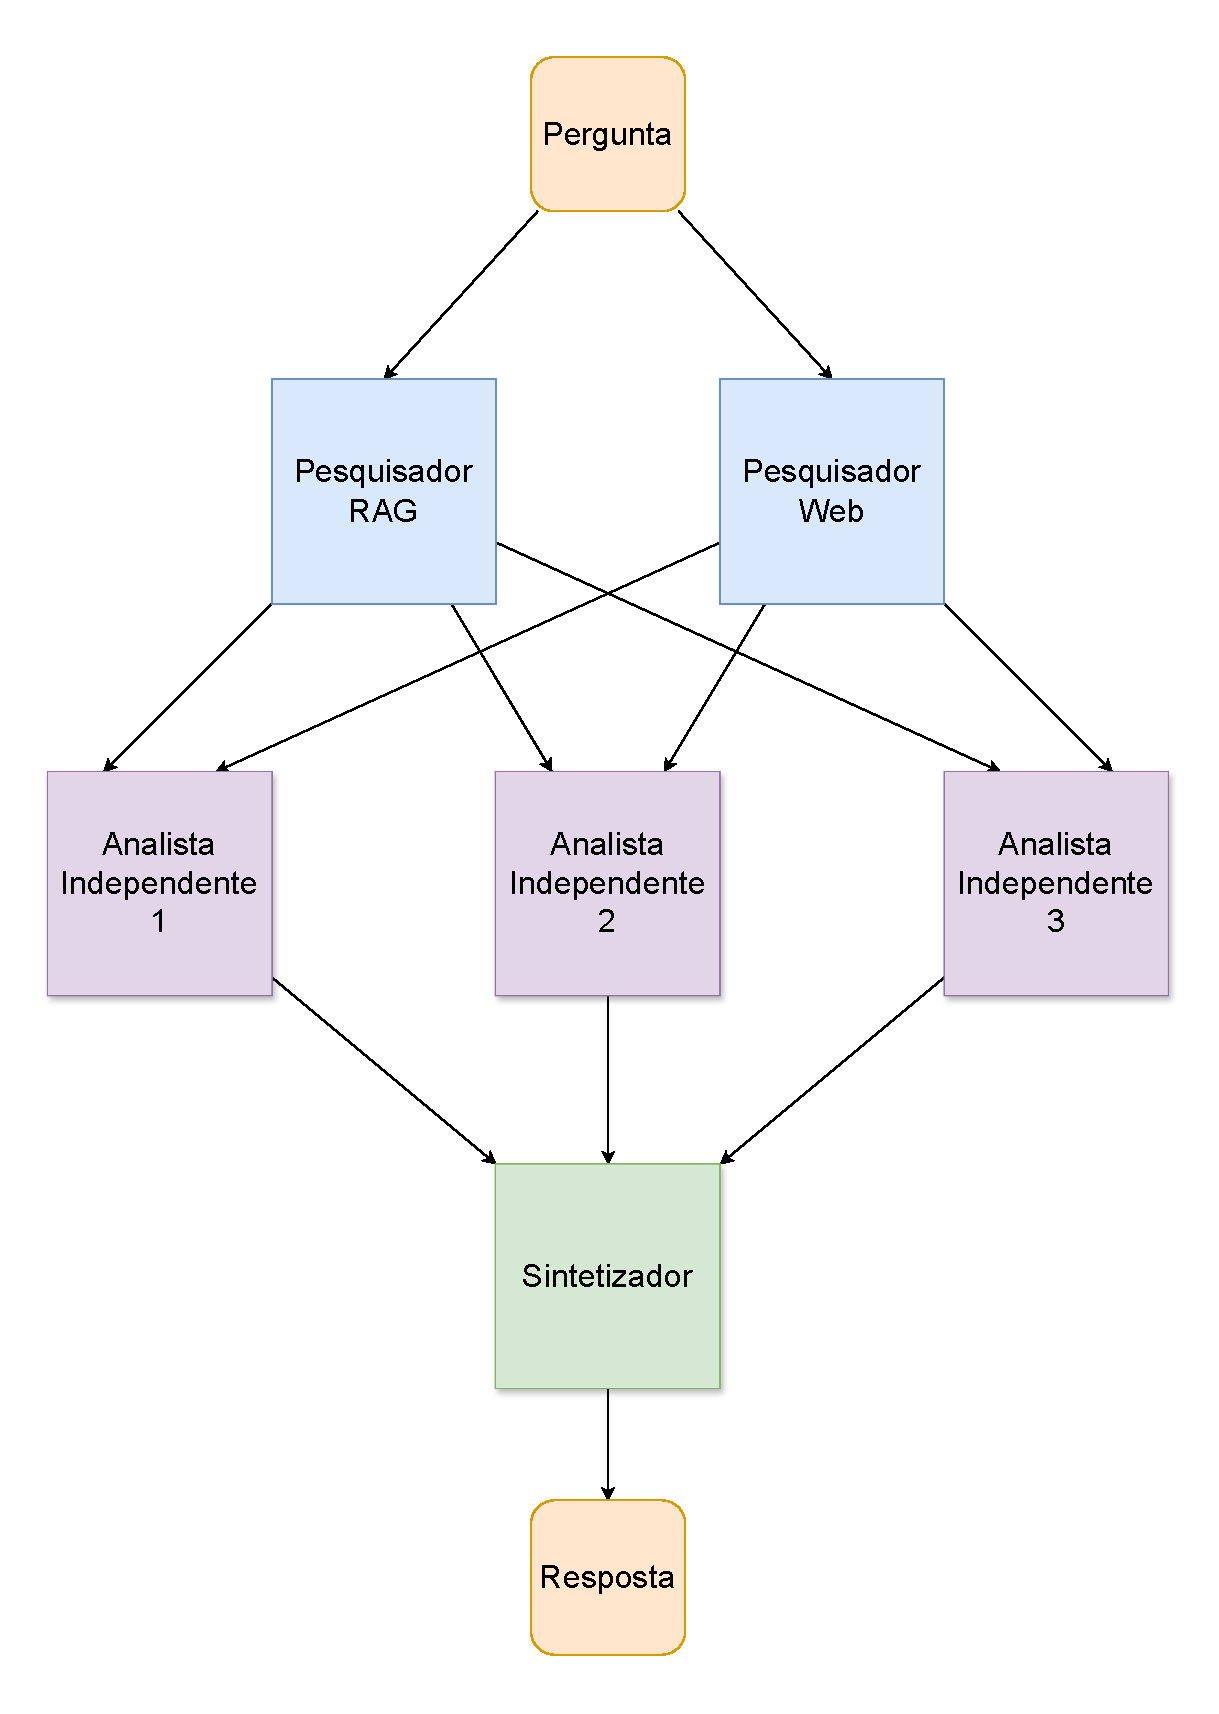
\includegraphics[width=0.6\textwidth]{resources/diagrama_custom_tp4.pdf}
    \caption{Fluxograma da arquitetura do sistema. }
    \label{fig:fluxo1}
\end{figure}

\begin{figure}[htpb]
    \centering
    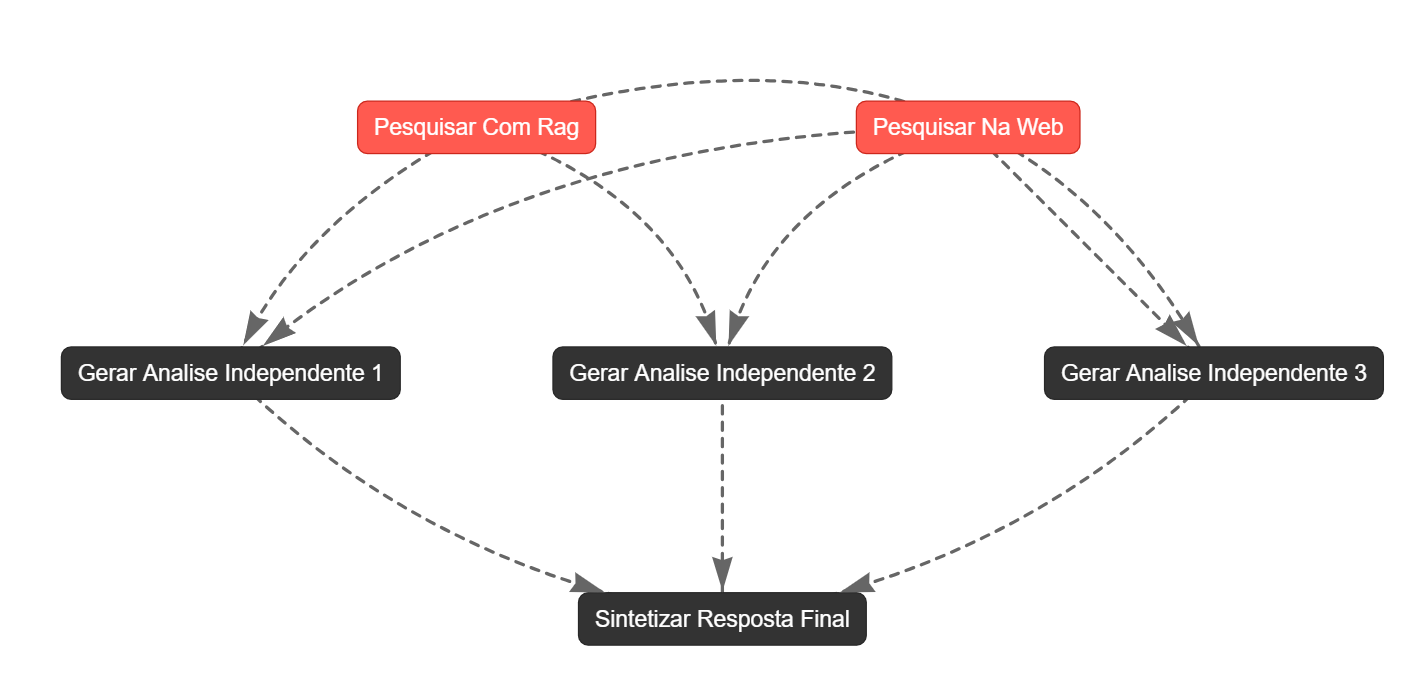
\includegraphics[width=\textwidth]{resources/diagrama_crewai.png}
    \caption{Fluxograma da arquitetura do sistema pelo CrewAI. }
    \label{fig:fluxo2}
\end{figure}
\end{document}